%%%%%%%%%%%%%%%%% DO NOT CHANGE HERE %%%%%%%%%%%%%%%%%%%% {
	\documentclass[10pt,a4]{article}
	\DeclareMathSizes{10}{10}{5.5}{4}
	\usepackage{makecell}
	\usepackage{enumerate}
	\usepackage{tcolorbox}%box宏包
	\tcbuselibrary{most}
	\usepackage{xcolor}
	\usepackage{graphicx}
	\usepackage{listings}
	\usepackage{hyperref}
	\usepackage{ctex}
	\usepackage{tikz}
	\usepackage{geometry}%页边距调整
	\geometry{left=2cm,right=2cm,bottom=2.8cm,top=2cm}
	\usepackage{newtxtext}
	\usepackage{newtxmath,bm}
	\usepackage{titlesec}
	\usepackage{fancyhdr}
	\usepackage{booktabs}
	\usepackage{makeidx}%索引专用
	
	\definecolor{titlepurple}{HTML}{5758BB}%一级标题(目前:蓝紫色)
	\definecolor{titlepurpleb}{HTML}{3A006F}%二级标题(目前:深紫色)
	\definecolor{titlepurplec}{HTML}{006266}%三级标题(目前:墨绿色)
	\definecolor{tab1}{HTML}{9698ED}%表格1
	\definecolor{tab2}{HTML}{DBDCFF}%表格2
	\definecolor{dy0}{HTML}{EA7500}%小标题定义专用(目前:橙黄色)
	\definecolor{dl}{HTML}{007500}%小标题定理专用(目前:深绿色)
	\definecolor{inference}{HTML}{343300}%小标题推论专用(目前:墨绿色)
	\definecolor{ex}{HTML}{7158e2}%小标题例专用(目前:紫色)
	\definecolor{dy}{HTML}{BF0060}%夹杂在文本中的定义词的颜色1(目前:深红色)
	\definecolor{dy2}{HTML}{FF0000}%夹杂在文本中的定义词的颜色2(目前:红紫色)
	\definecolor{dya}{HTML}{FFFFFF}
	\definecolor{超链接}{HTML}{0000C6}%含超链接的文字专用色(目前:蓝紫色)
	\definecolor{文字底色}{HTML}{F8FF00}%强调的文字底色(目前:黄色)
	\definecolor{eq}{HTML}{F0F0F0}
	\definecolor{tl}{HTML}{D94600}
	
	\titleformat{\section}{\bfseries\Large\color{titlepurple}}{第 \ \thesection\  章\quad }{0pt}{}
	\titleformat{\subsection}{\large\bfseries\color{titlepurplec}}{\thesubsection\ \quad  }{0pt}{}
	\titlespacing{\subsection}{0em}{0.1em}{0.3em}[1em]
	%格式如下:\titlespacing*{章节名称}{左间距}{(前)行间距}{(后)行间距}[右间距(一般都没用,填0.1em即可,但不能不填)]
	\titlespacing*{\subsubsection}{1.5em}{0.5em}{0.3em}[0em]
	\numberwithin{equation}{section}
	
	\hypersetup{%
		colorlinks=true,
		linkcolor=blue,
		linkbordercolor={0 0 1}
	}
	
	\setCJKmainfont[BoldFont={PingFangSC-Medium}]{PingFangSC-Regular}
	\setlength{\parindent}{0.0in}
	\setlength{\parskip}{0.05in}
	%%%%%%%%%%%%%%%%%%%%%%%%%%%%%%%%%%%%%%%%%%%%%%%%%%%%%%%%%% }

% %%%%%%%%%%%%%%%%%%%%%%%% CHANGE HERE %%%%%%%%%%%%%%%%%%%% {
	% %Margins and Header/Footer
	% \geometry{a4paper,
		%   top=2in,
		%   bottom=1.5in,
		%   left=1.5in,
		%   right=1in,
		%   headheight=14.5pt, % the default is too short
		%   heightrounded, % avoids the need of a flexible baselineskip
		% } 
	% %%%%%%%%%%%%%%%%%%%%%%%%%%%%%%%%%%%%%%%%%%%%%%%%%%%%%%%%%% }

%%%%%%%%%%%%%%%%%%%%%%%% CHANGE HERE %%%%%%%%%%%%%%%%%%%% {
	\newcommand\course{\Large \textcolor[rgb]{0.12,0.33,0.12}{\textbf{结构力学}}}
	\newcommand\semester{\large \textcolor[rgb]{0.12,0.33,0.12}{2021 年秋季学期}}
	\newcommand\SchoolLogo{
\includegraphics[scale=0.35]{./pic/SYSU_SAA_Logo.pdf}}
	%%%%%%%%%%%%%%%%%%%%%%%%%%%%%%%%%%%%%%%%%%%%%%%%%%%%%%%%%% }

%%%%%%%%%%%%%%%%% DO NOT CHANGE HERE %%%%%%%%%%%%%%%%%%%% {
	\pagestyle{fancyplain}
	\headheight 30pt
	\rhead{	
		\quad \\[1em]
		\begin{minipage}[l]{0.39\linewidth}
			\hspace*{-1em}
			\SchoolLogo
		\end{minipage}
		\begin{minipage}[r]{0.6\linewidth}
			\hspace*{24em}
			\course \\[0.2em]
			\hspace*{14.7em}\semester
		\end{minipage}\\[-1.1em]} 
	\setlength{\headsep}{3.5em}
	\setlength{\footskip}{2.5em}
	\renewcommand{\headrulewidth}{0mm}
	\rfoot{\textcolor[rgb]{0.12,0.33,0.12}{\small \bfseries 弹性力学基础笔记}}
	\cfoot{\textcolor[rgb]{0.12,0.33,0.12}{\small \bfseries \thepage}} 
	\lfoot{\textcolor[rgb]{0.12,0.33,0.12}{\small \bfseries 2019级航空航天工程专业本科}} 
	
	\renewcommand{\d}{\text{d}}
	\def\degree{{}^{\circ}}
	%%%%%%%%%%%%%%%%%%%%%%%%%%%%%%%%%%%%%%%%%%%%%%%%%%%%%%%%%% }

\title{\huge \bf
	弹性力学基础笔记
}
\author{19320125 \hspace*{1em} 易鹏}

%定义计数器
\newcounter{theorem}[section]
\newcounter{defination}[section]
\renewcommand{\thetheorem}{{ 定理} \textbf{\thesection.\arabic{theorem}}}
\renewcommand{\thedefination}{{ 定义} \textbf{\thesection.\arabic{defination}}}
\newcommand{\sj}{\hspace*{-2.7em}}
\newcommand{\red}[1][]{\textcolor{red}{#1}}

\newcommand{\mybox}[2][]{
	\begin{tcolorbox}[on line,
		arc=0pt,outer arc=0pt,colback=#1!10!white,colframe=#1,
		boxsep=0pt,left=3pt,right=3pt,top=6pt,bottom=6pt,
		boxrule=0pt,leftrule=1.5pt]#2
\end{tcolorbox}}

%定理类
\newcommand{\theorem}[2][]{\vspace{1em} \refstepcounter{theorem} \mybox[dl]{{\color{dl}\thetheorem\hspace{1em}#1}\\[0.1em] \hspace*{2em}#2}\vspace{0.5em} \par}

%定义类
\newcommand{\defination}[2][]{\vspace{1em} \refstepcounter{defination} \mybox[dy0]{{\color{dy0}\thedefination\hspace{1em}#1}\\[0.1em] \hspace*{2em}#2}\vspace{0.5em} \par}

%% 定义索引类
\newcommand{\dy}[2][]{{\color{dy}#1}\index{#2@#1}}
\newcommand{\dya}[2][]{\vspace*{0.7em} \noindent \tcbox[colframe =Chocolate , colback =Coral,boxrule=0.5mm,size=small,on line]{\color{dya}{\textbf{#1}}}  \index{#2@#1} \hspace*{1em}}
\newcommand{\dyb}[1][]{\vspace*{0.7em} \noindent \tcbox[colframe =Chocolate, colback =Coral,boxrule=0.5mm,size=small,on line]{\color{dya}{\textbf{#1}}} \hspace*{1em} }

%注意
\newcommand{\warn}[1][]{
	\vspace*{0.5em}
	\begin{tcolorbox}[colframe=red!75!black, colback=yellow!10!white,title=注意,fonttitle = ]
		#1
\end{tcolorbox}}
\newcommand{\summarize}[1][]{
	\vspace*{0.5em}
	\begin{tcolorbox}[colframe=white!20!black, colback=white!98!black,title=评注,fonttitle = ]
		#1
\end{tcolorbox}}

%文档开始
\begin{document}
	%标题及目录
	\maketitle
	\section{引言}
	\subsection{研究内容}
	\noindent 弹性力学是固体力学的分支,其研究对象为\vspace*{-0.5em}
	\begin{itemize}
		\item 材料力学研究杆状弹性体在拉伸、压缩、剪切、弯曲和扭转作用下的变形和内力。\vspace*{-0.5em}
		\item 弹性力学研究的对象为连续体,没有形状限制。 
	\end{itemize}
	研究方法为:\vspace*{-0.5em}
	\begin{itemize}
		\item 材料力学除了采用一些基本假设外,还引进一些关于变形状态或应力分布的补充假设。\vspace*{-0.5em}
		\item 弹性力学并不需要引进这样的补充假设。
	\end{itemize}
	
	弹性力学的研究方法更为严瑾,所得的结果也比材料力学精确,也常常用弹性力学的方法来评估材料力学方法的精度和适用范围。\vspace*{1em}
	
	
	\subsection{弹性力学的基本假设}
	\vspace*{-1em}
	\theorem[连续性假设(continuous)假设 ]
	{
		\index{LXXJS@连续性假设}构成物体的材料是密实无间隙的连续介质,并在变形过程中保持连续性。物体中的应力、应变、位移等物理量可以看成是连续的,在数学上可以用空间位置的连续函数表示。
	}
	
	\theorem[均匀性(homogeneous)假设]
	{
		\index{JYXJS@均匀性假设}物体内各处材料的力学性质都相同,与各点的空间位置无关。
	}
	
	\theorem[各向同性(isotropic)假设 ]
	{
		\index{GXTXJS@各向同性假设}在物体内任一点处材料在各个方向的物理性质都相同。反映这些物理性质的弹性系数不随坐标位置和方向而改变。
	}
	
	\theorem[完全线弹性(linear elasticity)假设 ]
	{
		\index{WQXTXJS@完全线弹性假设}假设材料是完全弹性的,且服从虎克定律,物体在外力作用下变形,除去外力后,物体完全恢复原状,没有任何剩余变形。应力与应变关系是线性的。
	}
	
	\theorem[小变形(small deformation / small deflection)假设 ]
	{
		\index{XBXJS@小变形假设}假设物体在外力作用下引起变形是微小的,与物体最小特征尺寸相比可以忽略不计。在研究物体受力后的平衡状态时,可不考虑物体尺寸的变化,而应用变形前的尺寸;研究变形时,变形的二次幂和乘积项都是高阶小量,可略去。这样就使得弹性力学的微分方程成为线性的。
	}
	
	\subsection{弹性力学中的基本概念}
	\vspace*{-1em}
	\defination[外力]
	{\dy[外力]{WL}:作用在物体上的力,可以分为体力和面力。\vspace*{-0.5em}
		{\begin{itemize}
				\item \dy[体力]{TL}:分布在物体整个体积的力,如重力、惯性力等。用体力沿坐标轴的投影表示。量纲为$[\mbox{力}][\mbox{长度}]^{-3}$,用$X,Y,Z$表示。\vspace*{-0.5em}
				
				\item \dy[面力]{ML}:作用于物体表面上的力,如流体压力、接触力等。用面力沿坐标轴的投影表示。量纲为$[\mbox{力}][\mbox{长度}]^{-3}$,用$\overline{X},\overline{Y},\overline{Z}$表示。
			\end{itemize}
		}
	}
	\begin{figure}[!thb]
		\centering
		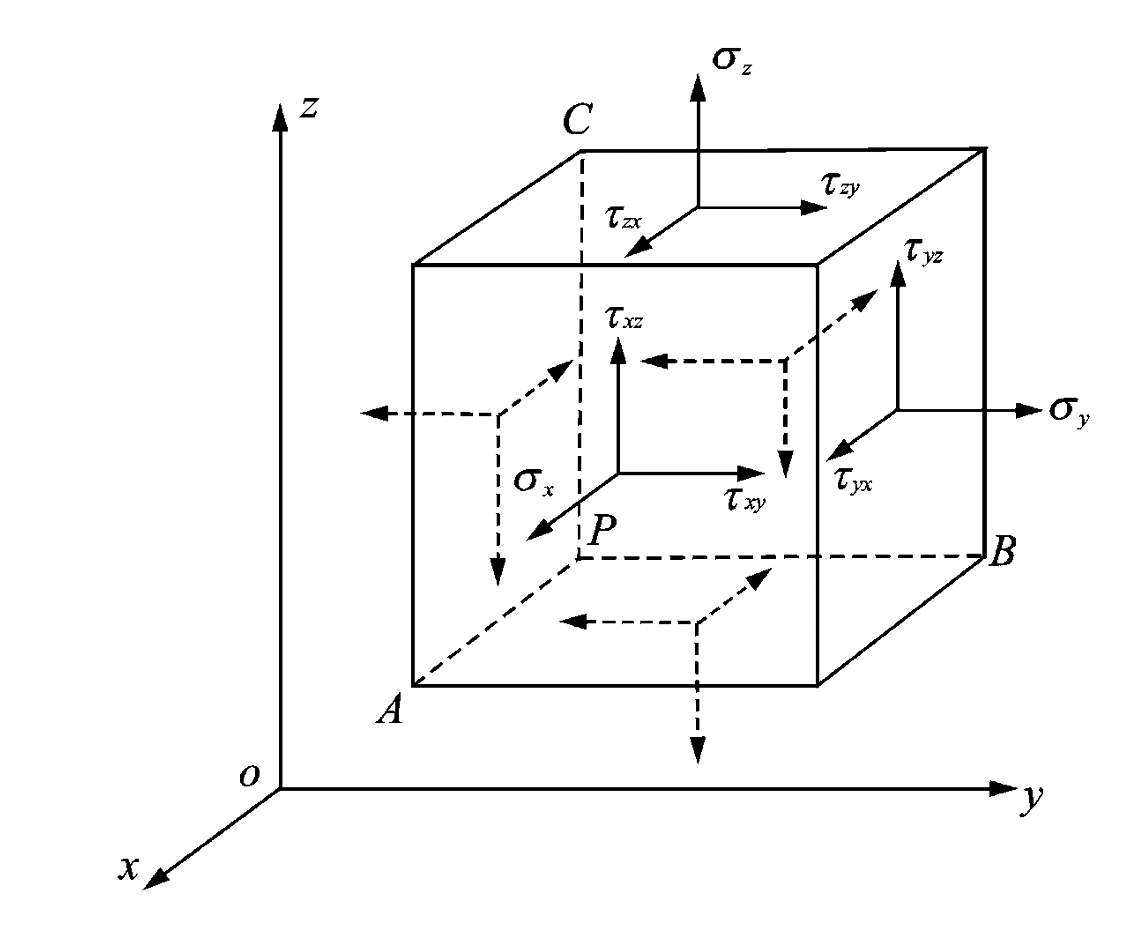
\includegraphics[width=0.5\linewidth]{pic/微元体.png}
		\caption{微元体示意图}
		\label{微元体}
	\end{figure}
	
	\defination[微元体]
	{\dy[微元体]{WYT}:宏观上足够小,微观上足够大。(如图\ref{微元体}所示)}
	
	\defination[应力(stress)]
	{\dy[应力]{YL}:物体收到外力作用会在其内部引起应力。}
	\vspace*{-0.5em}
	\begin{itemize}
		\item 每个面上有一个正应力和剪应力\vspace*{-0.5em}
		\item 正面上的应力沿坐标轴正向为正\vspace*{-0.5em}
		\item 负面上的应力沿坐标轴沿坐标轴负向为正\vspace*{-0.5em}
		\item 6个独立应力变量(剪应变互等定理)
		\begin{equation}
			\tau_{xy} = \tau_{yx}, \quad \tau_{yz} = \tau_{zy}, \quad \tau_{zx} = \tau_{xz}
		\end{equation}
	\end{itemize}
	
	\defination[应变(strain)]
	{
		\dy[应变]{YB}:弹性体受力后,他的形状和尺寸都要改变,这种改变可以归结为长度的改变和角度的改变。
	}
	\vspace*{-0.5em}
	\begin{itemize}
		\item 各线段没单位长度的伸缩称为\dy[正应变]{ZYB},用$\varepsilon$表示。\vspace*{-0.5em}
		\item 每两线段之间支教的改变称为\dy[剪应变]{JYB},用$\gamma$表示。(注:直角$\, \to \,$锐角,$\gamma > 0$)
	\end{itemize}
	
	\defination[位移]
	{\dy[位移]{WY}:物体受力后,它内部各点将发生位置的移动。物体内任一点的位移用它在$x,y,z$三坐标轴上的投影$u,v,w$来表示,沿坐标轴正方向为正,反之为负。这三个投影称为该点的位移分量。 }
	\begin{figure}[!thb]
		\centering
		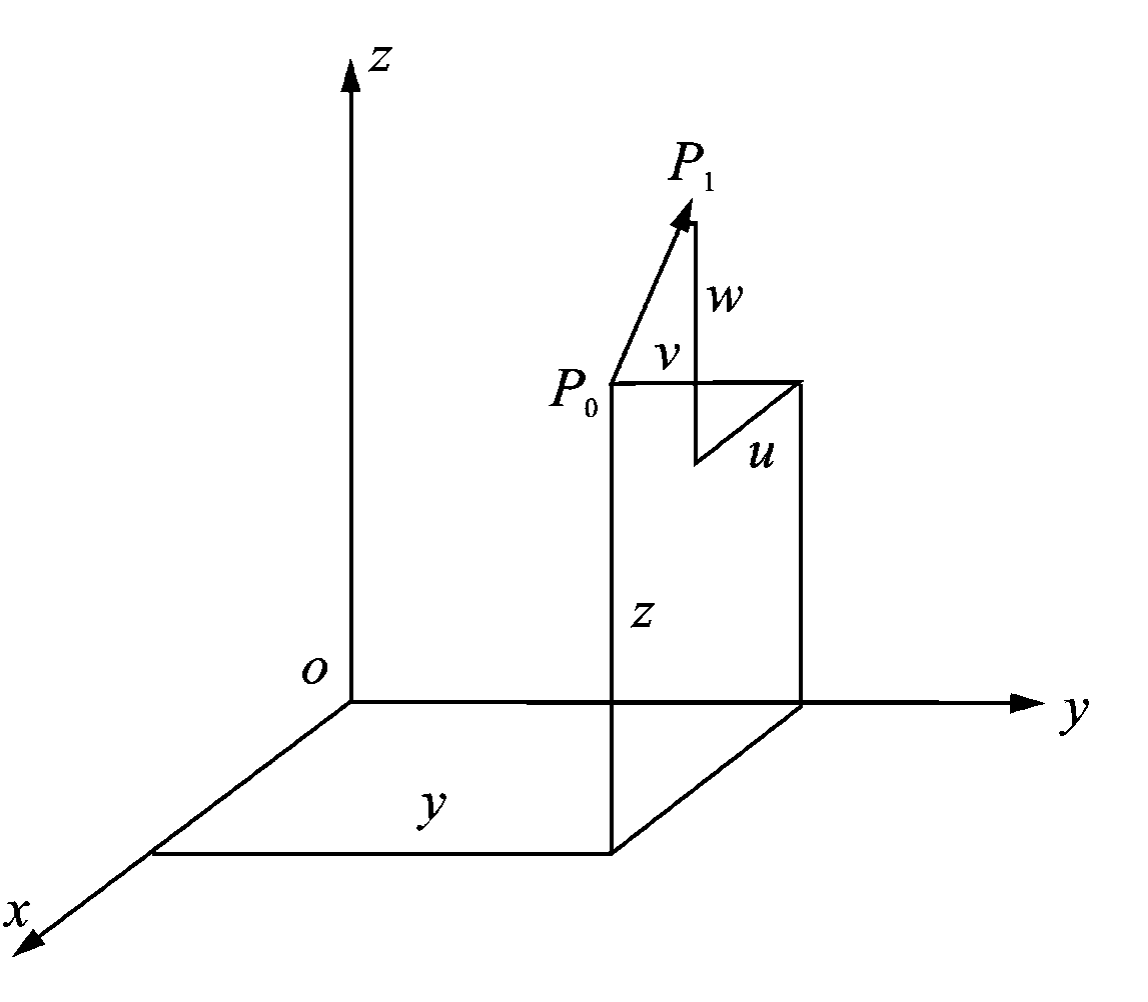
\includegraphics[width=0.35\linewidth]{pic/位移.png}
		\caption{位移示意图}
		\label{位移}
	\end{figure}
	
	\subsection{弹性力学的研究内容}
	一般而言,弹性体内任意点的体力分量、面力分量、应力分量、应变分量和位移分量都是随点的位置不同而改变的,因而,都是点位置坐标的连续函数(场函数)。
	
	弹性力学寻求建立连续体中体力、面力、应力场、应变场和位移场之间的关系。
	\vspace*{0.5em}
	
	\subsection{弹性力学的基本方法}
	采用微元体法,建立微分方程。\vspace*{-0.5em}
	\begin{itemize}
		\item \textbf{平衡方程}:外力—应力\vspace*{-0.5em}
		\item \textbf{几何方程}:位移—形变\vspace*{-0.5em}
		\item \textbf{物理方程}:应力—应变
	\end{itemize}
	
	\section{基本方程}
	建立微元体模型如图\ref{微元体应力}所示。
	
	\begin{figure}[!thb]
		\centering
		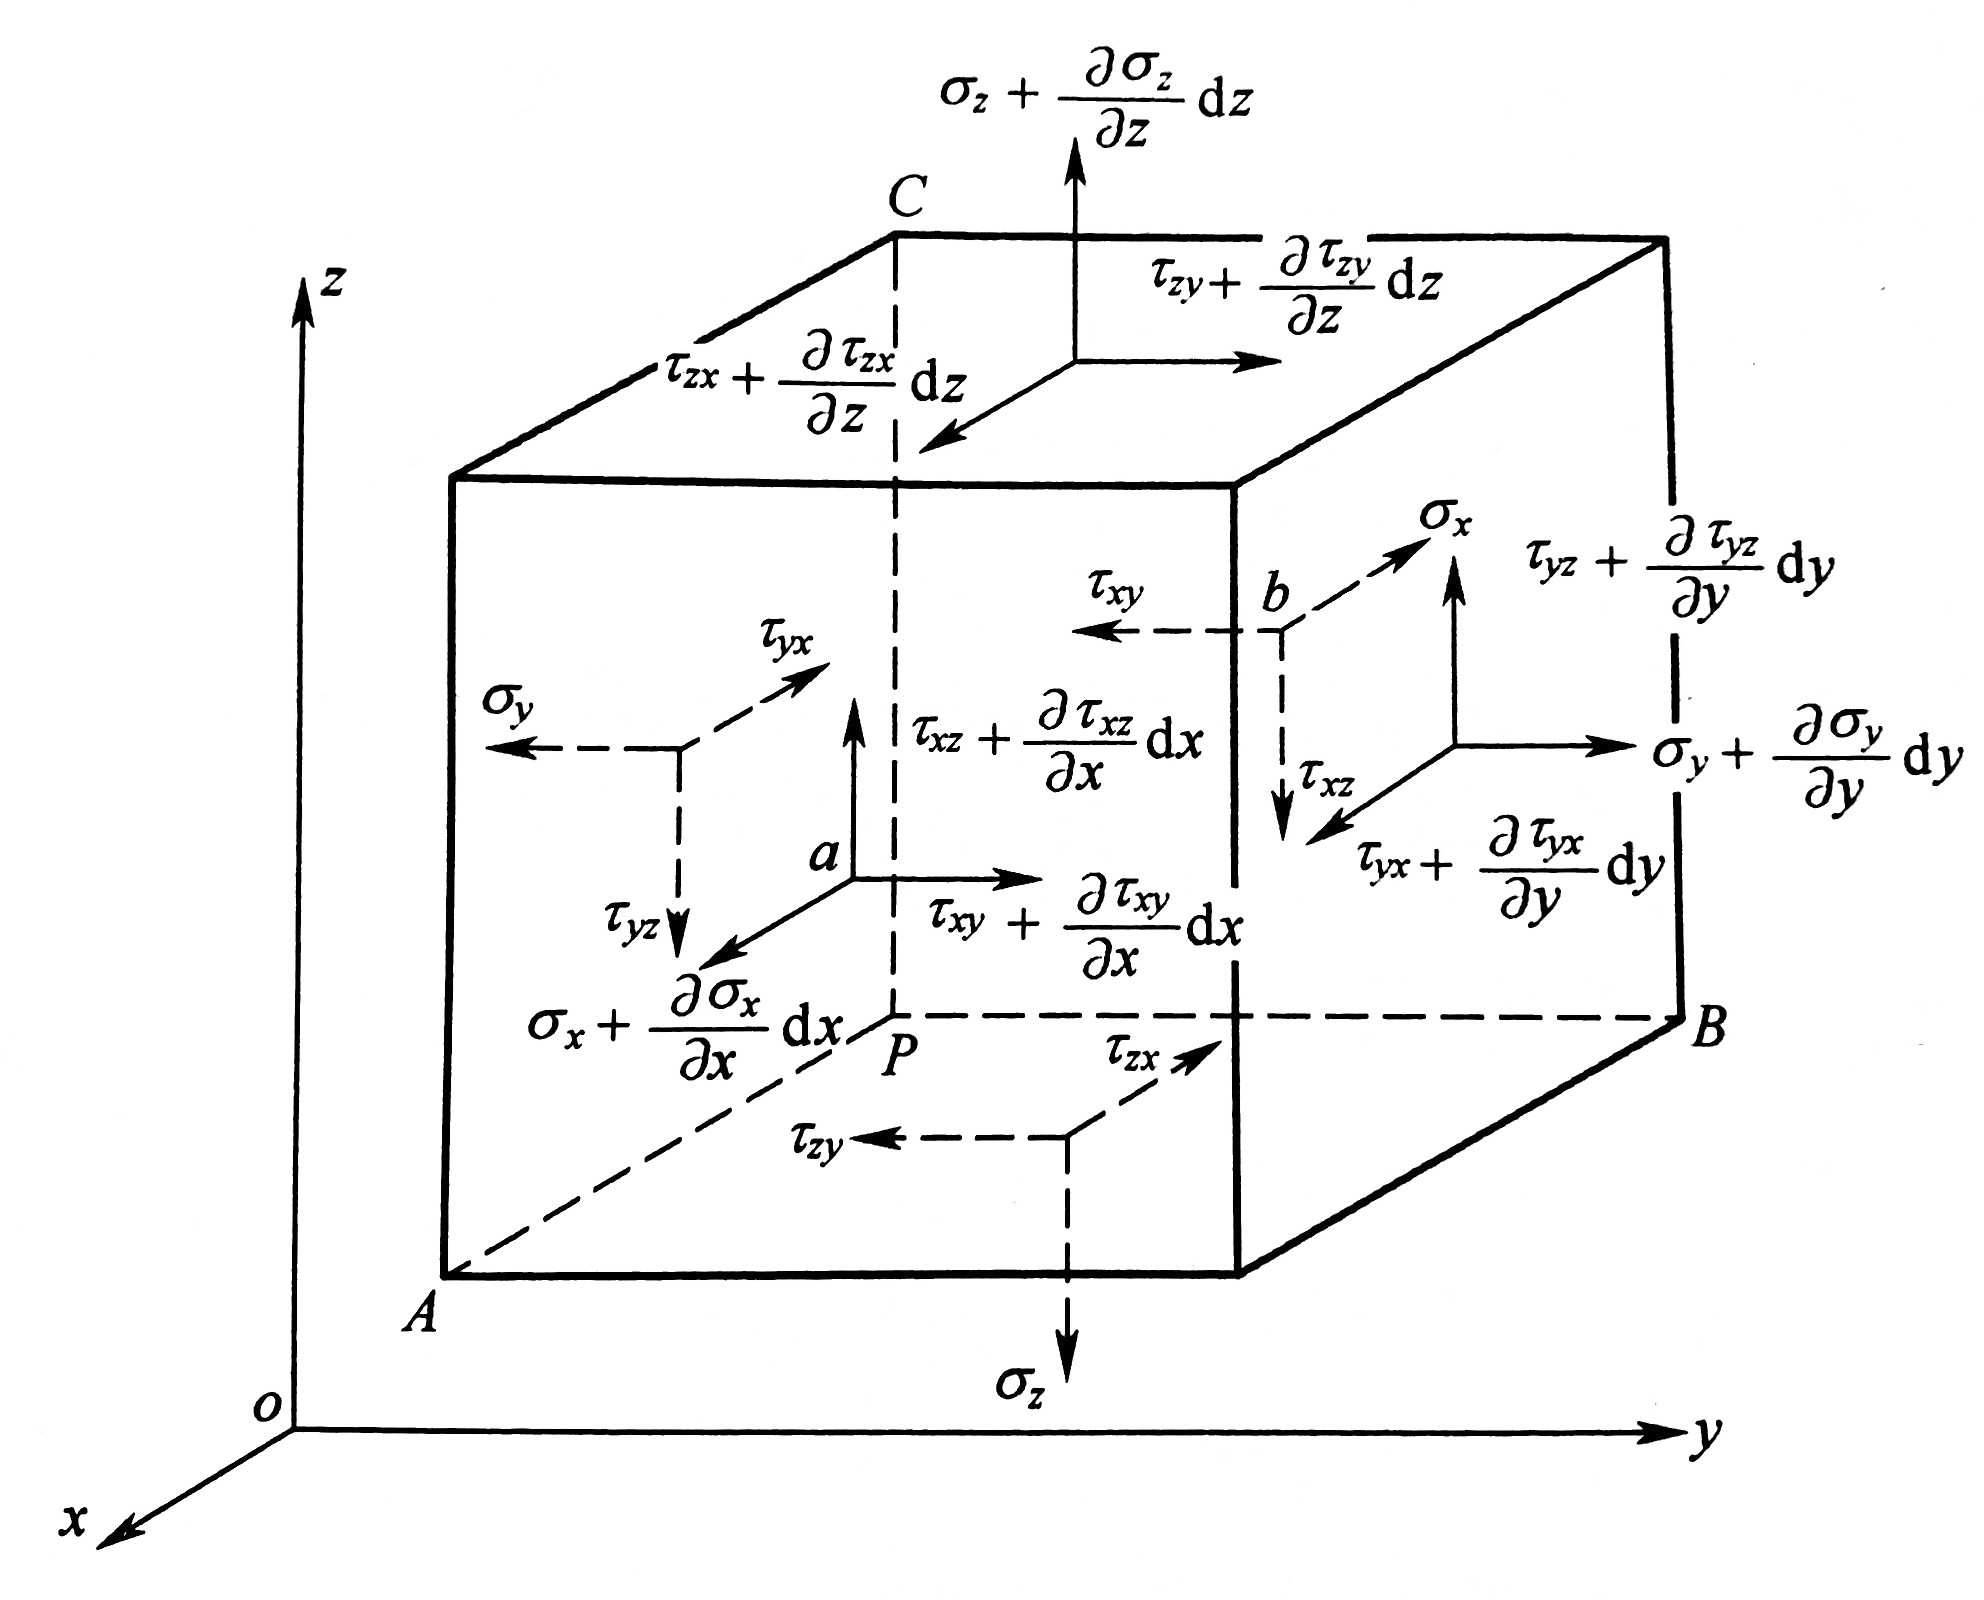
\includegraphics[width=0.6\linewidth]{pic/微元体应力.png}
		\caption{微元体应力模型}
		\label{微元体应力}
	\end{figure}
	
	\subsection{力平衡微分方程}
	如图\ref{微元体应力}所示,由力平衡,对$x$方向分析可得$\sum F_x = 0$,即
	\begin{equation}
		\left(\sigma_x + \dfrac{\partial \sigma_x}{\partial x}\, \d x\right)\d y \d z - \sigma_x \d y \d z + \left(\tau_{yx}+ \dfrac{\partial \tau_{yx}}{\partial y}\, \d y\right)\d x \d z - \tau_{yx}\,\d x \d z + \left(\tau_{zx} + \dfrac{\partial \tau_{zx}}{\partial z}\, \d z\right)\d x \d y - \tau_{zx}\d x \d y + X \d x \d y \d z = 0
	\end{equation}
	化简得
	\begin{equation}
		\begin{aligned}[c]
			\dfrac{\partial \sigma_x}{\partial x}\, \d x\d y \d z + \dfrac{\partial \tau_{yx}}{\partial y}&\, \d y \d x \d z + \dfrac{\partial \tau_{zx}}{\partial z}\, \d z \d x \d y + X \d x \d y \d z = 0 \\
			\dfrac{\partial \sigma_x }{\partial x} &+ \dfrac{\partial \tau_{yx}}{\partial y} + \dfrac{\partial \tau_{zx}}{\partial z} + X = 0
		\end{aligned}
	\end{equation}
	同理可以得到$y,z$方向上的力平衡方程,从而确定微元体的\dy[力平衡方程]{LPHFC}。
	
	\theorem[力平衡方程]
	{
		\quad \vspace*{-1em}
		\begin{equation}
			\begin{cases}
				\, \dfrac{\partial \sigma_x }{\partial x} + \dfrac{\partial \tau_{yx}}{\partial y} + \dfrac{\partial \tau_{zx}}{\partial z} + X = 0\\[0.7em]
				\, \dfrac{\partial \tau_{xy} }{\partial x} + \dfrac{\partial \sigma_{y}}{\partial y} + \dfrac{\partial \tau_{zy}}{\partial z} + Y = 0\\[0.7em]
				\, \dfrac{\partial \tau_{xz} }{\partial x} + \dfrac{\partial \tau_{yz}}{\partial y} + \dfrac{\partial \sigma_{z}}{\partial z} + Z = 0
			\end{cases}
			\label{力平衡}
		\end{equation}
	}
	
	\subsection{力矩平衡方程}
	如图\ref{微元体应力}所示,由力矩平衡,对$x$轴力矩有$\sum M_x = 0$,即
	\begin{equation}
		\left(\tau_{yz} + \dfrac{\partial \tau_{yz}}{\partial y}\, \d y\right)\, \d x \d z \dfrac{\d y}{2} + \tau_{yz}\, \d x \d z \dfrac{\d y}{2} - \left(\tau_{zy} + \dfrac{\partial \tau_{zy}}{\partial z}\, \d z\right)\d x \d y \dfrac{\d z}{2} - \tau_{zy}\, \d x \d y \dfrac{\d z}{2} = 0
	\end{equation}
	化简得
	\begin{equation}
		\dfrac{\partial \tau_{yz}}{\partial y}\, \d y \d x \d z \dfrac{\d y}{2} + \tau_{yz}\, \d x \d z \d y- \dfrac{\partial \tau_{zy}}{\partial z}\, \d z \d x \d y \dfrac{\d z}{2} - \tau_{zy} \, \d x \d y \d z = 0
	\end{equation}
	略去无穷小量,可得
	\begin{equation}
		\tau_{yz} = \tau_{zy}
	\end{equation}
	
	同理可以得到$y,z$方向上的力矩平衡方程,得到\dy[剪应力互等定律]{JYLHDDL}。
	
	\theorem[剪应力互等定律]
	{
		\quad \vspace*{-1em}
		\begin{equation}
			\tau_{yz} = \tau_{zy} \qquad \tau_{zx} = \tau_{xz} \qquad \tau_{xy} = \tau_{yx}
		\end{equation}
	}
	
	\subsection{几何方程}
	变形前,微元体在$xoy$面上的投影如图\ref{BX1}所示。变形后,微元体在$xoy$面上的投影如图\ref{BX2}。需要注意的是$u(x,y),v(x,y)$是双变量函数,不要看它们只是单方向的位移而忽视了这点。对于图中的量,设$P'(x,y)$,则$A''(x+\d x, y), B'' (x, y + \d y)$,取泰勒一阶展开式:
	$$ \left. PA' \right|_{x} = u(x, y) + u_x (x + \d x - x) = u + \dfrac{\partial u}{\partial x} \d x \qquad \left. PA' \right|_{y} = v(x, y) + v_x (x + \d x - x) = v + \dfrac{\partial v}{\partial x} \d x$$
	\vspace*{-1em}
	
	\begin{figure}[!htb]
		\begin{minipage}{0.5\linewidth}
			\centering
			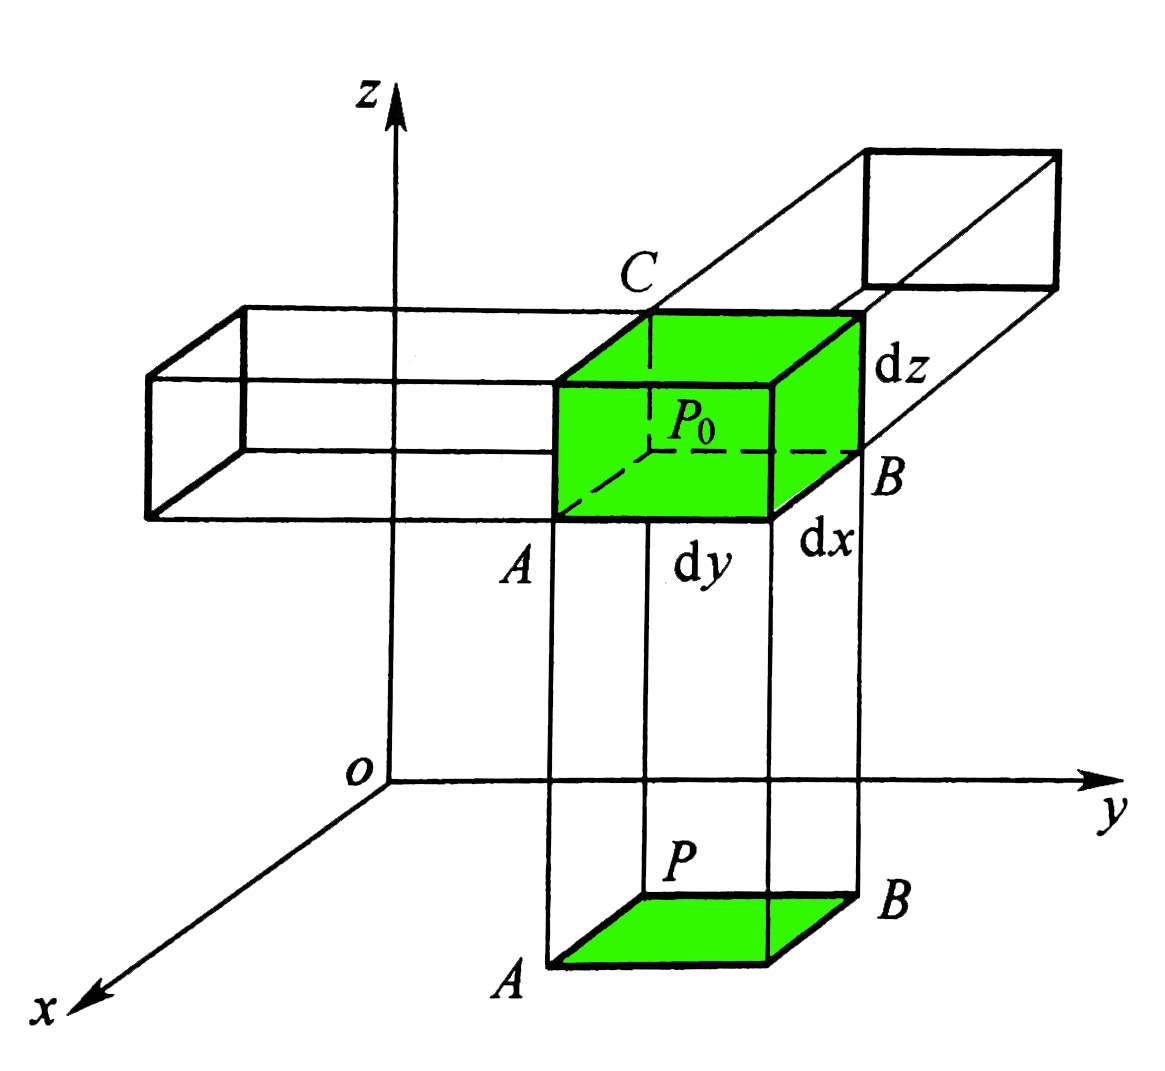
\includegraphics[width=0.8\linewidth]{pic/变形1.png}
			\caption{变形前微元体投影示意图}
			\label{BX1}
		\end{minipage}
		\begin{minipage}{0.5\linewidth}
			\centering
			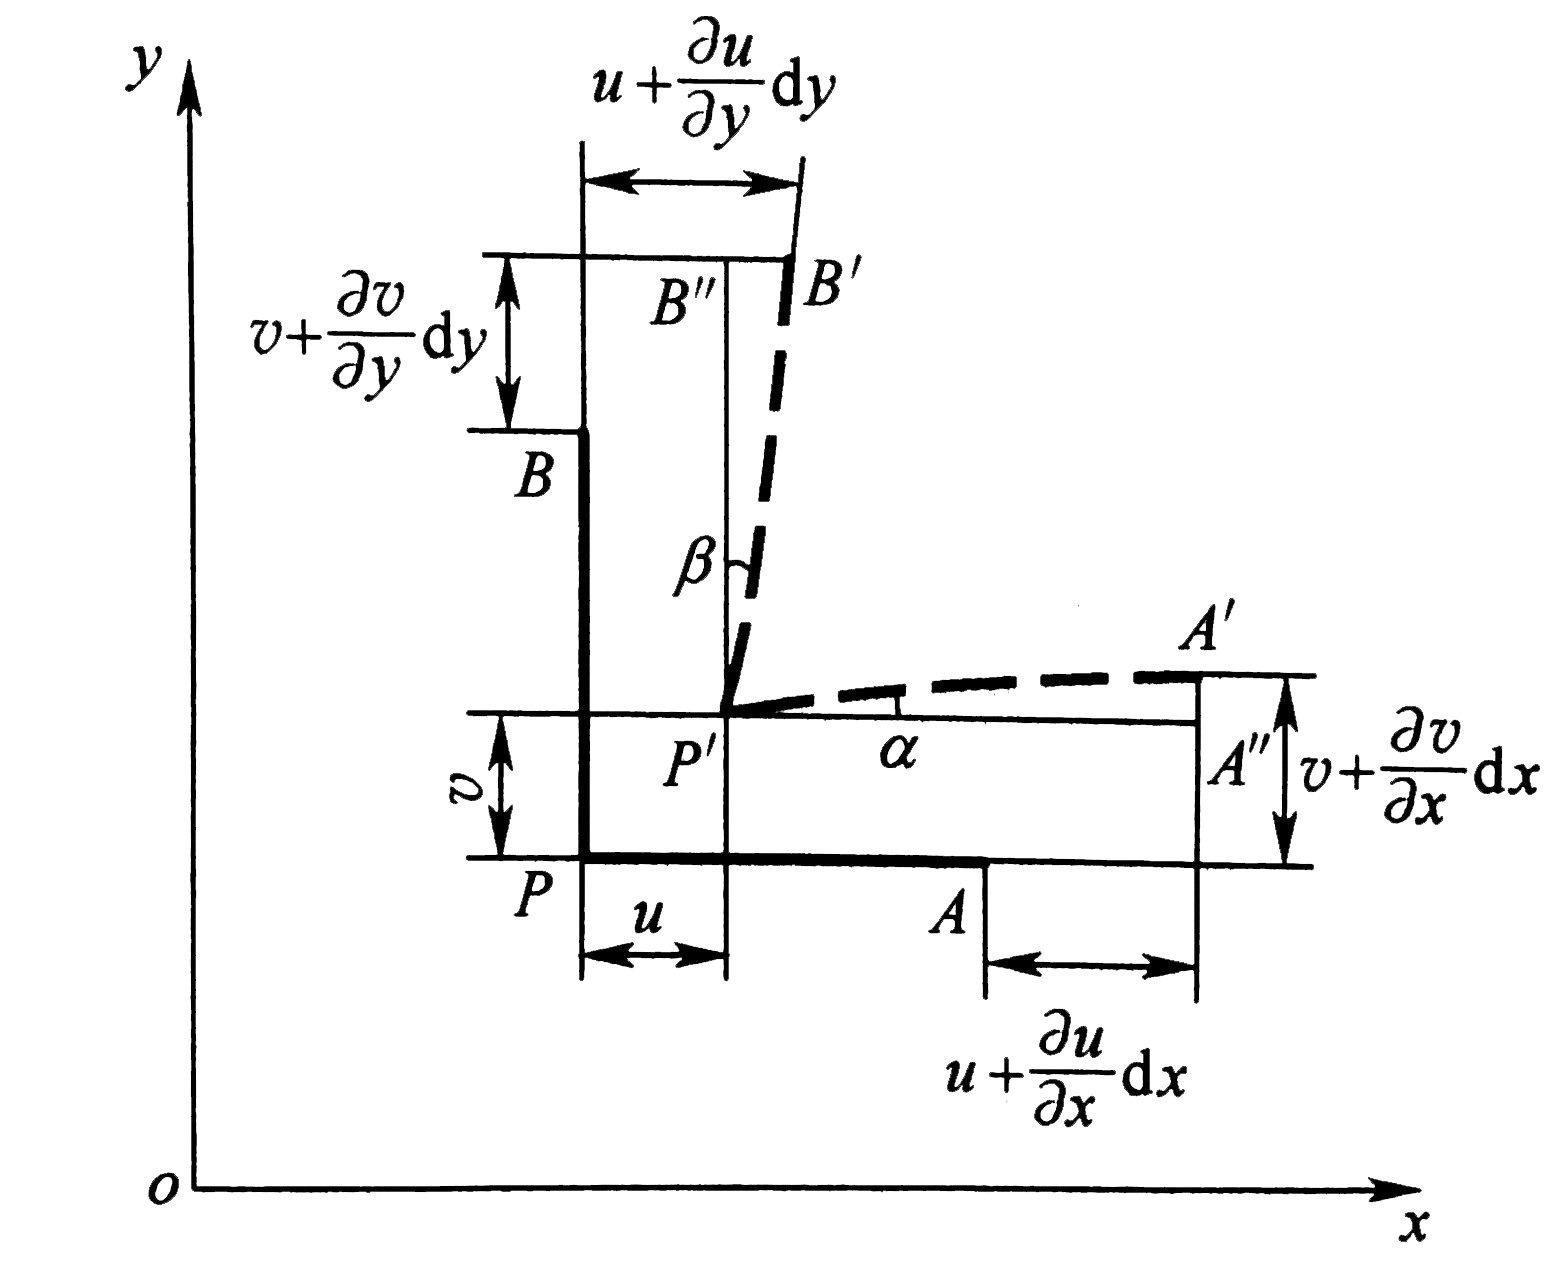
\includegraphics[width=0.9\linewidth]{pic/变形2.png}
			\caption{变形后微元体投影示意图}
			\label{BX2}
		\end{minipage}
	\end{figure}
	
	则线段$PA$的正应变为
	\begin{equation}
		\varepsilon_x = \dfrac{P'A' - PA}{PA} \approx \dfrac{P'A'' - PA}{PA} = \dfrac{u + \dfrac{\partial u}{\partial x}\,\d x - u}{\d x} = \dfrac{\partial u}{\partial x}
	\end{equation}
	同理可得
	\begin{equation}
		\varepsilon_y = \dfrac{\partial v}{\partial y}, \qquad \varepsilon_z = \dfrac{\partial w}{\partial z}
	\end{equation}
	
	而点$P_0$处的剪应变为线段$PA$和线段$PB$之间直角的改变,其包括$PA$向$y$轴方向的转角$\alpha$,另一部分是$PB$向$x$轴方向的转角$\beta$。在小变形情况下,有
	\begin{equation}
		\alpha \approx \tan \alpha = \dfrac{A'A''}{P'A''} = \dfrac{\dfrac{\partial v}{\partial x}\, \d x}{\d x + \dfrac{\partial u}{\partial x}\, \d x} = \dfrac{\dfrac{\partial v}{\partial x}}{1 + \dfrac{\partial u}{\partial x}}
	\end{equation}
	
	而由于$\dfrac{\partial u}{\partial x} = \varepsilon_x \ll 1$,可以略去。则进一步化简为
	\begin{equation}
		\alpha = \dfrac{\partial v}{\partial x}
	\end{equation}
	同理,可以得到
	\begin{equation}
		\beta \approx \tan \beta = \dfrac{B'B''}{P'B''} = \dfrac{\dfrac{\partial u}{\partial y}\, \d y}{\d y + \dfrac{\partial v}{\partial y}\,\d y} = \dfrac{\partial u}{\partial y}
	\end{equation}
	从而得到切应变为
	\begin{equation}
		\tau_{xy} = \alpha + \beta = \dfrac{\partial v}{\partial x} + \dfrac{\partial u}{\partial y}
	\end{equation}
	同理分析$xoz,yoz$平面上的投影变化,可以得到相应的切应变为
	\begin{equation}
		\gamma_{yz} = \dfrac{\partial w}{\partial y} + \dfrac{\partial v}{\partial z}, \qquad \gamma_{zx} = \dfrac{\partial u}{\partial z} + \dfrac{\partial w}{\partial x}
	\end{equation}
	综合分析结果,可以得到\dy[几何方程]{JHFC}。
	
	
	\theorem[几何方程(应变—位移关系式)]
	{
		\quad \vspace*{-1em}
		\begin{equation}
			\begin{cases}
				\, \varepsilon_x = \dfrac{\partial u}{\partial x}, & \gamma_{yz} = \dfrac{\partial w}{\partial y} + \dfrac{\partial v}{\partial z}\\[0.7em]
				\varepsilon_y = \dfrac{\partial v}{\partial y}, & \gamma_{zx} = \dfrac{\partial u}{\partial z} + \dfrac{\partial w}{\partial x}\\[0.7em]
				\varepsilon_z = \dfrac{\partial w}{\partial z}, & \gamma_{xy} = \dfrac{\partial v}{\partial x} + \dfrac{\partial u}{\partial y}
			\end{cases}
			\label{JHFC}
		\end{equation}
	}
	
	\warn[\hspace*{1.75em} 当物体对位移分量给定时,应变分量就完全确定了。但是反过来,当应变分量给定时,\textcolor{red}{位移分量却不能完全确定},需要\textcolor{blue}{给定边界条件}。]
	\vspace*{0.5em}
	
	\subsection{刚体位移}
	\begin{enumerate}
		\item \textbf{平面刚体位移}\\
		\hspace*{1.75em} 对于平面刚体,结合几何方程\eqref{JHFC}有
		\begin{equation*}
			\varepsilon_x = \dfrac{\partial u}{\partial x} = 0, \qquad \varepsilon_y = \dfrac{\partial v}{\partial y} = 0, \qquad \gamma_{xy} = \dfrac{\partial v}{\partial x} + \dfrac{\partial u}{\partial y} = 0
		\end{equation*}
		对前面两个式子进行积分,得到
		\begin{equation*}
			u = f_1 (y), \qquad v = f_2(x)
		\end{equation*}
		代入第三个式子,得
		\begin{equation*}
			- \dfrac{\d f_1(y)}{\d y} = \dfrac{\d f_2(x)}{\d x}
		\end{equation*}
		上式对左边是$y$的函数,右边是$x$的函数,所以只可能是常数,设这个常数为$\omega_z$即
		\begin{equation*}
			- \dfrac{\d f_1(y)}{\d y} = \omega_z, \qquad \dfrac{\d f_2(x)}{\d x} = \omega_z
		\end{equation*}
		积分后可得
		\begin{equation}
			\begin{cases}
				\, u = f_1(y) = u_0 - \omega_z y\\
				\, v = f_2(x) = v_0 + \omega_z x
			\end{cases}
		\end{equation}
		其中,$u_0$和$v_0$是积分常量。对于结果里面的各参数,都有其物理意义。$u_0,v_0$分别代表$x,y$方向的平动;$\omega_z$代表刚体绕$z$轴的转动。
		
		\item \textbf{空间刚体位移}\\
		\hspace*{1.75em} 对于空间刚体,和平面刚体类似,可以得到
	\end{enumerate}
	
	\theorem[空间刚体位移]
	{
		\begin{equation}
			\begin{cases}
				\, u = u_0 + \omega_y z  - \omega_z y\\
				\, v = v_0 + \omega_z x - \omega_x z\\
				\, w = w_0 +\omega_x y - \omega_y x
			\end{cases}
		\end{equation}
		其中,$u_0,v_0,w_0$分别代表$x,y,z$方向的平动;$\omega_x, \omega_y, \omega_z$代表刚体绕$x,y,z$轴的转动。
	}
	
	由此可知,应变为0时,弹性体仍可能存在刚体位移,为此引入位移边界条件的概念。
	
	\defination[位移边界条件]
	{ 
		当物体发生一定的形变时,由于约束条件的不同,它可能具有不同的位移,为了确定物体的位移,消除物体的刚体位移,必须有足够的约束条件,这些条件称为\dy[位移边界条件]{WYBJTJ},即
		\begin{equation}
			\begin{cases}
				\, u = \overline{u}\\
				\, v = \overline{v}\\
				\, w = \overline{w}
			\end{cases}
		\end{equation}
	}
	
	
	\subsection{变形协调方程}
	
	由几何方程可见,六个应变分量完全由三个位移分量对坐标对偏导数所确定。因此这六个变量不是相互独立的,它们之间一定存在关系。由于关系式均有轮换对称性,在推导时只列举一种情况。
	\begin{itemize}
		\item 第一组关系
		\begin{equation*}
			\dfrac{\partial^2 \varepsilon_x}{\partial y^2} + \dfrac{\partial^2 \varepsilon_y}{\partial x^2} = \dfrac{\partial^2 }{\partial y^2}\left(\dfrac{\partial u}{\partial x}\right) + \dfrac{\partial^2}{\partial x^2}\left(\dfrac{\partial v}{\partial y}\right) = \dfrac{\partial^2 }{\partial x \partial y} \left(\dfrac{\partial u}{\partial y} + \dfrac{\partial v}{\partial x}\right) = \dfrac{\partial^2 \gamma_{xy}}{\partial x \partial y}
		\end{equation*}
		
		\item 第二组关系
		\begin{equation*}
			\dfrac{\partial \gamma_{yz}}{\partial x} + \dfrac{\partial \gamma_{xz}}{\partial y} - \dfrac{\partial \gamma_{xy}}{\partial z} = \dfrac{\partial }{\partial x}\left(\dfrac{\partial w}{\partial y} + \dfrac{\partial v}{\partial z}\right) + \dfrac{\partial }{\partial y} \left(\dfrac{\partial u}{\partial z} + \dfrac{\partial w}{\partial x}\right) - \dfrac{\partial }{\partial z}\left(\dfrac{\partial v}{\partial x} + \dfrac{\partial u}{\partial y}\right) = 2 \dfrac{\partial^2 w}{\partial x \partial y}
		\end{equation*}
		对上式对$z$求导数,得到
		\begin{equation*}
			\dfrac{\partial }{\partial z}\left(\dfrac{\partial \gamma_{yz}}{\partial x} + \dfrac{\partial \gamma_{xz}}{\partial y} - \dfrac{\partial \gamma_{xy}}{\partial z}\right) = 2 \dfrac{\partial^2}{\partial x \partial y}\left(\dfrac{\partial w}{\partial z}\right) = 2 \dfrac{\partial^2 \varepsilon_z}{\partial x \partial y}
		\end{equation*}
	\end{itemize}
	两组关系汇集,得到\dy[变形协调方程]{BXXTFC}。
	
	\theorem[变形协调方程]
	{
		\begin{equation}
			\begin{cases}
				\, \dfrac{\partial^2 \varepsilon_x}{\partial y^2} + \dfrac{\partial^2 \varepsilon_y}{\partial x^2} = \dfrac{\partial^2 \gamma_{xy}}{\partial x \partial y}, & \dfrac{\partial }{\partial x}\left(\dfrac{\partial \gamma_{zx}}{\partial y} + \dfrac{\partial \gamma_{xy}}{\partial z} - \dfrac{\partial \gamma_{yz}}{\partial x}\right) = 2 \dfrac{\partial^2 \varepsilon_x}{\partial y \partial z} \\[0.9em]
				
				\, \dfrac{\partial^2 \varepsilon_y}{\partial z^2} + \dfrac{\partial^2 \varepsilon_z}{\partial y^2} = \dfrac{\partial^2 \gamma_{yz}}{\partial y \partial z}, & \dfrac{\partial }{\partial y}\left(\dfrac{\partial \gamma_{xy}}{\partial z} + \dfrac{\partial \gamma_{yz}}{\partial x} - \dfrac{\partial \gamma_{zx}}{\partial y}\right) = 2 \dfrac{\partial^2 \varepsilon_y}{\partial z \partial x} \\[0.9em]
				
				\, \dfrac{\partial^2 \varepsilon_z}{\partial x^2} + \dfrac{\partial^2 \varepsilon_x}{\partial z^2} = \dfrac{\partial^2 \gamma_{zx}}{\partial z \partial x}, & \dfrac{\partial }{\partial z}\left(\dfrac{\partial \gamma_{yz}}{\partial x} + \dfrac{\partial \gamma_{xz}}{\partial y} - \dfrac{\partial \gamma_{xy}}{\partial z}\right) = 2 \dfrac{\partial^2 \varepsilon_z}{\partial x \partial y}
			\end{cases}
		\end{equation}
	}
	
	\section{物理方程}
	
	平衡微分方程和几何方程,适用于任何弹性体,与物体的物理性质无关。
	但仅有这两组方程还不能求解,还必须考虑物理学方面。
	
	\defination[物理方程(Physical Equations)]
	{
		建立起应变分量与应力分量之间的关系,这些关系式称为\dy[物理方程]{WLFC}。 
		\begin{equation}
			\begin{cases}
				\, \sigma_x = C_{11}\varepsilon_x + C_{12} \varepsilon_y + C_{13}\varepsilon_z + C_{14}\gamma_{yz} + C_{15} \gamma_{zx} + C_{16} \gamma_{xy}\\
				\, \sigma_y = C_{21}\varepsilon_x + C_{22} \varepsilon_y + C_{23}\varepsilon_z + C_{24}\gamma_{yz} + C_{25} \gamma_{zx} + C_{26} \gamma_{xy}\\
				\, \sigma_z = C_{31}\varepsilon_x + C_{32} \varepsilon_y + C_{33}\varepsilon_z + C_{34}\gamma_{yz} + C_{35} \gamma_{zx} + C_{36} \gamma_{xy}\\
				\tau_{yz} = C_{41}\varepsilon_x + C_{42} \varepsilon_y + C_{43}\varepsilon_z + C_{44}\gamma_{yz} + C_{45} \gamma_{zx} + C_{46} \gamma_{xy}\\
				\tau_{zx} = C_{51}\varepsilon_x + C_{52} \varepsilon_y + C_{53}\varepsilon_z + C_{54}\gamma_{yz} + C_{55} \gamma_{zx} + C_{56} \gamma_{xy}\\
				\tau_{xy} = C_{61}\varepsilon_x + C_{62} \varepsilon_y + C_{63}\varepsilon_z + C_{64}\gamma_{yz} + C_{65} \gamma_{zx} + C_{66} \gamma_{xy}\\
			\end{cases}
		\end{equation}
		写成矩阵形式为
		\begin{equation}
			\begin{bmatrix}
				\sigma_x \\
				\sigma_y \\
				\sigma_z \\
				\tau_{yz} \\
				\tau_{zx} \\
				\tau_{xy}
			\end{bmatrix}
			=
			\begin{bmatrix}
				C_{11} & C_{12} & C_{13} & C_{14} & C_{15} & C_{16}\\
				C_{21} & C_{22} & C_{23} & C_{24} & C_{25} & C_{26}\\
				C_{31} & C_{32} & C_{33} & C_{34} & C_{35} & C_{36}\\
				C_{41} & C_{42} & C_{43} & C_{44} & C_{45} & C_{46}\\
				C_{51} & C_{52} & C_{53} & C_{54} & C_{55} & C_{56}\\
				C_{61} & C_{62} & C_{63} & C_{64} & C_{65} & C_{66}
			\end{bmatrix}
			\begin{bmatrix}
				\varepsilon_x & \varepsilon_y & \varepsilon_z & \tau_{yz} & \tau_{zx} & \tau_{xy}
			\end{bmatrix}
		\end{equation}
	}
	
	
	对于各向同性弹性体,仅有两个独立的弹性常数,其应变分量与应力分量之间的关系如下:
	
	\theorem[广义胡克定律\index{GYHKDL@广义胡克定律}]
	{
		\quad \vspace*{-1em}
		\begin{equation}
			\begin{cases}
				\, \varepsilon_x = \dfrac{1}{E} \big[\sigma_x - \mu (\sigma_y + \sigma_z) \big], & \gamma_{yz} = \dfrac{\tau_{yz}}{G}\\[0.7em]
				
				\, \varepsilon_y = \dfrac{1}{E} \big[\sigma_y - \mu (\sigma_z + \sigma_x) \big], & \gamma_{zx} = \dfrac{\tau_{zx}}{G}\\[0.7em]
				
				\, \varepsilon_z = \dfrac{1}{E} \big[\sigma_z - \mu (\sigma_x + \sigma_y) \big], & \gamma_{xy} = \dfrac{\tau_{xy}}{G}
			\end{cases}
		\end{equation}
		其中,$E$为材料\dy[拉压弹性模量]{LYTXML},$\mu$为\dy[泊松比]{PSB},$G$为\dy[剪切弹性模量]{JQTXML},而且三者之间的关系为
		\vspace*{-0.5em}
		\begin{equation}
			G = \dfrac{E}{2(1 + \mu)}
		\end{equation}
	}
	
	若用应变分量来表示应力分量,其物理方程为
	\begin{equation}
		\begin{split}
			&\begin{cases}
				\, \sigma_x = \lambda e + 2 G \varepsilon_x, & \tau_{yz} = G \gamma_{yz} \\
				\, \sigma_y = \lambda e + 2 G \varepsilon_y, & \tau_{zx} = G \gamma_{zx} \\
				\, \sigma_z = \lambda e + 2 G \varepsilon_z, & \tau_{xy} = G \gamma_{xy}
			\end{cases}	\\[0.5em]
			e = \varepsilon_x + \varepsilon_y + \varepsilon_z, &\qquad \lambda = \dfrac{E\mu}{(1 + \mu)(1 - 2\mu)}, \qquad G = \dfrac{E}{2(1 + \mu)}
		\end{split}
	\end{equation}
	
	\section{应力边界条件和圣维南原理}
	
	\subsection{应力边界条件}
	物体处于平衡状态时,除了满足平衡方程\eqref{力平衡},在物体边界上还受到外部载荷的作用,借此可以得到应力分量和面力分量的关系。
	
	取一个正六面微元体,到了物体边界上,就变成来正四面体$P-ABC$,其体积为$\d V = \dfrac{1}{3}\, \d A \cdot \d h.$记斜微分面$ABC$的外法线方向为$\bm{N}$,其与各坐标轴夹角的方向余弦分别为
	\begin{equation*}
		l = \cos (\bm{N}, \bm{x}),\qquad m = \cos (\bm{N}, \bm{y}), \qquad n = \cos (\bm{N}, \bm{z})
	\end{equation*}
	斜微分面$ABC$上的面力沿三个坐标轴上的投影分别为$\overline{X}, \overline{Y}, \overline{Z}$.由于微分面很小,其面上作用的应力和面力可看作均匀分布的。考虑$x$方向上的受力,由受力平衡,有
	\begin{equation}
		\overline{X}\d A -\sigma_x l \d A-\tau_{yx} m \d A - \tau_{zx} n \d A + X \d V= 0
	\end{equation}
	消去高阶小量$X \d V$并化简得到
	\begin{equation}
		l \sigma_x + m \tau_{yx} + n \tau_{zx} = \overline{X}
	\end{equation}
	类似地,$y,z$方向受力平衡综合得到
	
	\theorem[应力边界条件]
	{
		\quad \vspace*{-1em}
		\begin{equation}
			\begin{cases}
				\, l \sigma_x + m\tau_{yx} + n \tau_{zx} = \overline{X} \\
				\, l \tau_{xy} + m \sigma_y + n\tau_{zy} = \overline{Y} \\
				l \tau_{xz} + m \tau_{yz} + n \sigma_{z} = \overline{Z}
			\end{cases}
		\end{equation}
	}
	
	\section{平面应力和平面应变问题}
	\begin{table}[!htb]
		\centering
		\setlength{\tabcolsep}{6mm}{
			\begin{tabular}{ccc}
				\hline 
				& 平面应力问题 & 平面应变问题 \\
				\hline
				几何特点 & 等厚度板,厚度远小于板的长度 & 纵向尺寸远大于横向尺寸 \\
				\hline
				受力特点 & \makecell[c]{面力、体力平行于板平面\\且沿板厚均匀分布} & \makecell[c]{面力、体力垂直纵向且沿长度不变,\\约束条件沿长度也不变} \\
				\hline
				应力、应变特点 & \makecell[c]{只有面内应力$\sigma_x,\sigma_y,\tau_{xy}$存在,\\应变$\varepsilon_z$和位移$w$不为0} & \makecell[c]{只有面内应变分量$\varepsilon_x, \varepsilon_y, \gamma_{xy}$存在,\\应力$\sigma_{z} $不为0}\\
				\hline
			\end{tabular}
		}
	\end{table}
	\subsection{平面问题的基本方程}
	\begin{enumerate}
		\item \textbf{平衡方程}
		\begin{equation}
			\begin{cases}
				\, \dfrac{\partial \sigma_x }{\partial x} + \dfrac{\partial \tau_{yx}}{\partial y}  + X = 0\\[0.7em]
				\, \dfrac{\partial \tau_{xy} }{\partial x} + \dfrac{\partial \sigma_{y}}{\partial y} + Y = 0
			\end{cases}
			\label{平面平衡方程}
		\end{equation}
		
		\item \textbf{力边界条件}
		\begin{equation}
			\begin{cases}
				\, l \sigma_x + m\tau_{yx} = \overline{X} \\
				\, l \tau_{xy} + m \sigma_y = \overline{Y} 
			\end{cases}
		\end{equation}
		
		\item \textbf{几何方程}
		\begin{equation}
			\begin{cases}
				\, \varepsilon_x = \dfrac{\partial u}{\partial x}\\[0.7em]
				\, \varepsilon_y = \dfrac{\partial v}{\partial y} \\[0.7em]
				\, \tau_{xy} = \dfrac{\partial v}{\partial x} + \dfrac{\partial u}{\partial y}
			\end{cases}
			\label{平面几何方程}
		\end{equation}
		
		\item \textbf{变形协调方程}
		\begin{equation}
			\dfrac{\partial^2 \varepsilon_x}{\partial y^2} + \dfrac{\partial^2 \varepsilon_y}{\partial x^2} = \dfrac{\partial^2 \gamma_{xy}}{\partial x \partial y}
			\label{平面协调方程}
		\end{equation}
	\end{enumerate}
	
	\subsection{平面问题的物理方程}
	\begin{enumerate}
		\item \textbf{平面应力问题的物理方程}
		\begin{equation}
			\begin{cases}
				\varepsilon_x = \dfrac{1}{E}(\sigma_x - \mu \sigma_y) \\[0.7em]
				\varepsilon_y = \dfrac{1}{E}(\sigma_y - \mu \sigma_x)\\[0.7em]
				\gamma_{xy} = \dfrac{2(1+\mu)}{E}\tau_{xy}
			\end{cases}
			\qquad \qquad
			\begin{cases}
				\sigma_x = \dfrac{E}{1 - \mu^2}(\varepsilon_x + \mu \varepsilon_y)\\[0.7em]
				\sigma_{y} = \dfrac{E}{1 - \mu^2}(\varepsilon_y + \mu \varepsilon_x)\\[0.7em]
				\tau_{xy} = \dfrac{E}{2(1+\mu)}\gamma_{xy}
			\end{cases}
			\label{平面应力物理方程}
		\end{equation}
		
		\item \textbf{平面应变问题的物理方程}
		\begin{equation}
			\begin{cases}
				\varepsilon_x = \dfrac{1 -\mu^2}{E}(\sigma_x - \dfrac{\mu}{1 - \mu} \sigma_y) \\[0.7em]
				\varepsilon_y = \dfrac{1 - \mu^2}{E}(\sigma_y - \dfrac{\mu}{1-\mu} \sigma_x)\\[0.7em]
				\gamma_{xy} = \dfrac{2(1+\mu)}{E}\tau_{xy}
			\end{cases}
			\qquad \qquad
			\begin{cases}
				\, \sigma_x = \dfrac{E(1 - \mu)}{(1 + \mu)(1 -2\mu)}
				\left( \varepsilon_x + \dfrac{\mu}{1 - \mu} \varepsilon_y \right)
				\\[0.7em]
				\, \sigma_{y} = \dfrac{E(1 - \mu)}{(1 + \mu)(1 -2\mu)}
				\left(\varepsilon_y + \dfrac{\mu}{1 - \mu} \varepsilon_x \right)
				\\[0.7em]
				\, \tau_{xy} = \dfrac{E}{2(1+\mu)}\gamma_{xy}
			\end{cases}
		\end{equation}
	\end{enumerate}
	
	\subsection{平面问题的解法}
	\begin{enumerate}[\textbf{方法} 1 ]
		\item \textbf{位移法}\\
		\hspace*{1.75em} 以位移分量$u$和$v$作为基本未知函数,利用几何方程和物理方程,将应力分量用位移分量来表示,代入平衡微分方程、应力边界条件,就得到以位移分量为未知函数的定解方程、以及力边界条件。
		\red[工程上应用较少。]
		\begin{equation}
			\begin{cases}
				\, \varepsilon_x = \dfrac{\partial u}{\partial x}\\[0.7em]
				\, \varepsilon_y = \dfrac{\partial v}{\partial y} \\[0.7em]
				\, \tau_{xy} = \dfrac{\partial v}{\partial x} + \dfrac{\partial u}{\partial y}
			\end{cases}
			\quad
			\xrightarrow{\quad \mbox{代入平面应力问题的物理方程} \quad }
			\quad
			\begin{cases}
				\, \sigma_x = \dfrac{E}{1 - \mu^2}\left(\dfrac{\partial u}{\partial x} + \mu \dfrac{\partial v}{\partial y}\right)\\[0.7em]
				\, \sigma_y = \dfrac{E}{1 - \mu^2}\left(\dfrac{\partial v}{\partial y} + \mu \dfrac{\partial u}{\partial x}\right)\\[0.7em]
				\, \tau_{xy} = \dfrac{E}{2(1+\mu)} \left(\dfrac{\partial v}{\partial x} + \mu \dfrac{\partial v}{\partial y}\right)
			\end{cases}
		\end{equation}
		再代入力平衡方程,得到
		\begin{equation}
			\begin{cases}
				\, \dfrac{E}{1 - \mu^2}\left(\dfrac{\partial^2 u}{\partial x^2} + \dfrac{1 - \mu}{2}\dfrac{\partial^2 u}{\partial y^2} + \dfrac{1 + \mu}{2}\dfrac{\partial^2 v}{\partial x \partial y}\right) + X = 0 \\[0.8em]
				\, \dfrac{E}{1 - \mu^2}\left(\dfrac{\partial^2 v}{\partial y^2} + \dfrac{1 - \mu}{2}\dfrac{\partial^2 v}{\partial x^2} + \dfrac{1 + \mu}{2}\dfrac{\partial^2 u}{\partial x \partial y}\right) + Y = 0
			\end{cases}
		\end{equation}
		同样地,可以得到应力边界条件和位移边界条件:
		\begin{equation}
			\begin{cases}
				\dfrac{E}{1 - \mu^2}\left[l \left(\dfrac{\partial u}{\partial x} + \mu \dfrac{\partial v}{\partial y}\right) + m \dfrac{1-\mu}{2}\left(\dfrac{\partial u}{\partial y} + \dfrac{\partial v}{\partial x}\right)\right] = \overline{X} \\[0.8em]
				\dfrac{E}{1 - \mu^2}\left[m \left(\dfrac{\partial v}{\partial y} + \mu \dfrac{\partial u}{\partial x}\right) + l \dfrac{1-\mu}{2}\left(\dfrac{\partial v}{\partial x} + \dfrac{\partial u}{\partial y}\right)\right] = \overline{Y} 
			\end{cases}
		\end{equation}
		
		\item \textbf{应力法}\\
		\hspace*{1.75em} 以应力分量作为基本未知量,利用平衡微分方程和变形协调方程可共同确定这三个未知函数。在这三个方程中,两个平衡方程本来就是用应力分量表示的,尚需将应变分量表示的变形协调方程改为用应力分量表示,得到所需的第三个方程。 \\
		\hspace*{1.75em} 将物理方程\eqref{平面应力物理方程}代入变形协调方程\eqref{平面协调方程}可以得到
		\begin{equation}
			\dfrac{\partial^2}{\partial y^2} (\sigma_x - \mu \sigma_y) + \dfrac{\partial^2}{\partial x^2}(\sigma_y - \mu \sigma_x) = 2(1+\mu) \dfrac{\partial^2 \tau_{xy}}{\partial x \partial y}
		\end{equation}
		由平衡微分方程\eqref{平面平衡方程}消去上式中的$\tau_{xy}$,即
		
	\end{enumerate}
	
	%打印索引—————————————
	\clearpage
	\addcontentsline{toc}{chapter}{附录}
	\addcontentsline{toc}{section}{索引}
	\color{titlepurplec}
	\appendix
	\printindex
	%———————————————
\end{document}